\thispagestyle{empty}% Page de garde (FR)
\topskip1cm
\vspace*{\fill}
\begin{center}
{\Large \textbf{Cadre Analytique Modulaire pour l’Hypothèse de Riemann (T1$′$–T4)}}\\[6pt]
\textit{InterIA Mathematical Collective — Preuve-seule, prêt-journal, compatible arXiv}\\[12pt]
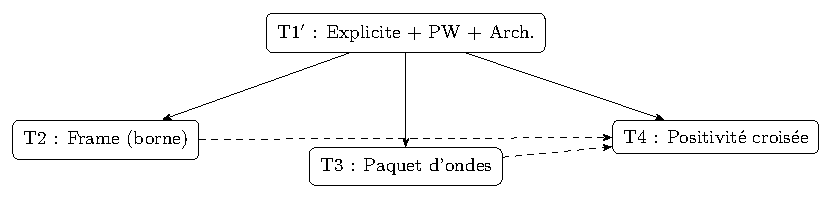
\includegraphics[width=.92\linewidth]{docs/explication-grand-format/latex/graphe_dependances_standalone_FR.pdf}\\[4pt]
\textbf{Carte de dépendances du schéma T1$'$–T4}
\end{center}
\vspace*{\fill}
%\clearpage
\pagebreak
